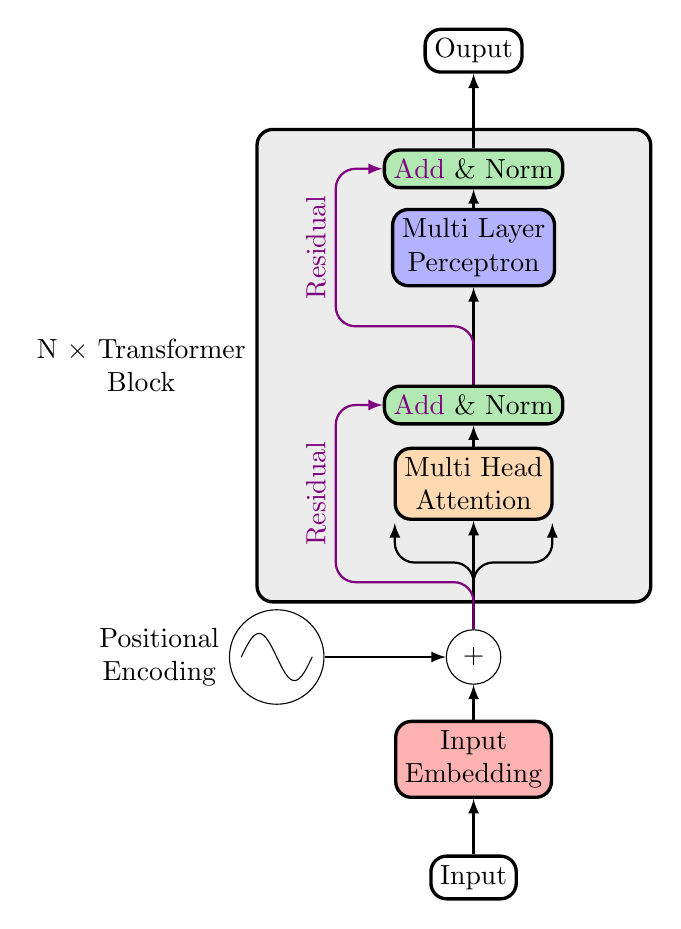
\begin{tikzpicture}[
	cell/.style={
		rectangle, 
		rounded corners=2mm, 
		draw,
		very thick,
		align=center,
	},
	ArrowC1/.style={% Arrows with rounded corners
		rounded corners=.25cm,
		thick,
	},
	do path picture/.style={%
		path picture={%
			\pgfpointdiff{\pgfpointanchor{path picture bounding box}{south west}}%
			{\pgfpointanchor{path picture bounding box}{north east}}%
			\pgfgetlastxy\x\y%
			\tikzset{x=\x/2,y=\y/2}%
			#1
		}
	},
	sin wave/.style={do path picture={    
			\draw [line cap=round] (-3/4,0)
			sin (-3/8,1/2) cos (0,0) sin (3/8,-1/2) cos (3/4,0);
	}},
]
	\node [cell] (out) at (0,10.5) {Ouput};
	
	\node [cell, fill=lightgray!30, minimum height=6cm, minimum width=5cm, label={[align=center]left:N $\times$ Transformer \\ Block}] (tb) at (-0.25,6.5) {};
	\node [cell, fill=black!30!green!30] (an2) at (0,9) {\textcolor{violet}{Add} \& Norm};
	\node [cell, fill=blue!30] (mlp) at (0,8) {Multi Layer \\ Perceptron};
	\node [cell, fill=black!30!green!30] (an1) at (0,6) {\textcolor{violet}{Add} \& Norm};
	\node [cell, fill=orange!30] (mha) at (0,5) {Multi Head \\ Attention};
	
	
	\node [draw, circle] (+) at (0,2.8) {$+$};
	\node [cell, fill=red!30] (emb) at (0,1.5) {Input \\ Embedding};
	\node [cell] (in) at (0,0) {Input};
	\node[circle, draw, sin wave, minimum size=1.2cm, label={[align=center]left:Positional \\ Encoding}] (pos) at (-2.5,2.8) {};
	
	\draw [-latex,ArrowC1] (in) -- (emb);
	\draw [-latex,ArrowC1] (emb) -- (+);
	\draw [-latex,ArrowC1] (+) -- (0,4) -- (mha);
	\draw [-latex,ArrowC1] (mha) -- (an1);
	\draw [-latex,ArrowC1] (an1) -- (0,7) -- (mlp);
	\draw [-latex,ArrowC1] (mlp) -- (an2);
	\draw [-latex,ArrowC1] (an2) -- (out);
	\draw [-latex, ArrowC1] (pos) -- (+);
	
	\draw [-latex, ArrowC1] (+) -- (0,4) -- (1,4) -- (1,4.5);
	\draw [-latex, ArrowC1] (+) -- (0,4) -- (-1,4) -- (-1,4.5);
	
	\draw [-latex, ArrowC1,violet] (+) -- (0,3.75) -- (-1.75, 3.75) -- (-1.75,3.5 |- an1) node[sloped,above,midway] {Residual} -- (an1);
	\draw [-latex, ArrowC1,violet] (an1) -- (0,7) -- (-1.75, 7) -- (-1.75,7 |- an2) node[sloped,above,midway] {Residual} -- (an2);
\end{tikzpicture}